\textbf{Judicious interpolation:} Repeat the above except that you interpolate at the roots of the Chebycheff polynomials, i.e. \[x_i = 5 \cos \frac{i \pi}{n},\;\;\; i=0,1,\dots,n.\]

{\color{blue}

\begin{figure}[H]
\centering
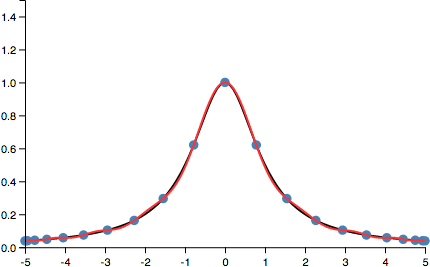
\includegraphics[scale=0.65]{runge-chebycheff.png}
\caption{We interpolate points obtained from the Runge function across
  an interval of points with $n=20$ made up from the Chebycheff roots
  in red. The original Runge function is plotted in black, along with
  the points we've interpolated from. Some minor fluctuation is
  visible, however it's overall much more accurate in our domain.}
\end{figure}

\begin{figure}[H]
\centering
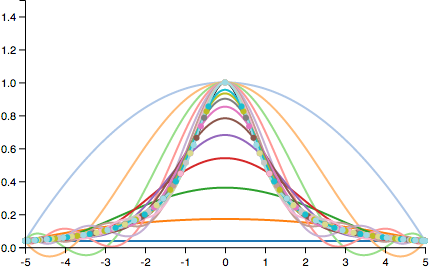
\includegraphics[scale=0.65]{runge-chebycheff-n-1-20.png}
\caption{Once again plotting several interpolations with
  $n=1,\dots,20$ we can see that all the functions interpolated with
  the Chebycheff roots behave much better than the previous problem
  with equidistant points.}
\end{figure}

Here we have that our interpolated polynomial still fluctuates near
the boundaries of our interpolation, but it behaves much better as the
points are distributed more at either end, and thus interpolated better.

}
